% DEFINED:   sec:exp-single-lookup, sec:multihead, sec:exp-multihop,
%            fig:ch06-grokking
% RESOLVED:  (none new)
% FORWARD:   (none)

\section{Experiment 1: depth on a single lookup}\label{sec:exp-single-lookup}

We train three models on the single-lookup task, all at comparable parameter
counts, all with Adam at learning rate $10^{-3}$ for 2000 iterations of batch
size 32. The code is \texttt{examples/pointer\_experiments.py}, and the
paired notebook regenerates these numbers.

\begin{center}
\begin{tabular}{@{}lrrrr@{}}
\toprule
Model & Layers & Heads & Parameters & Test accuracy \\
\midrule
MLP baseline & (n/a) & (n/a) & 3{,}018 & \textbf{1.000} \\
Transformer & 1 & 1 & 8{,}738 & 0.654 \\
Transformer & 2 & 1 & 17{,}282 & \textbf{1.000} \\
\bottomrule
\end{tabular}
\end{center}

Three things to read off this table. The \textbf{one-layer transformer
stalls} near 65 percent, modestly above the 50 percent chance line but
nowhere near the ceiling. That is exactly the structural prediction of
\Cref{sec:one-layer-limit}: the model can learn a fixed attention pattern and
pick up the single bit of information the address bit at position 10 already
carries, but it cannot do the dynamic lookup, and adding parameters within one
layer cannot fix an architectural limit.

The \textbf{two-layer transformer reaches 100 percent}, and it gets there with
a sharp phase transition rather than a smooth climb. The training loss sits at
the random line, $\ln 2 \approx 0.69$, for the first several hundred
iterations, then drops steeply, then settles at machine zero. The held-out
accuracy stays at chance through the plateau and then jumps to one over the
same short window. This is the grokking shape that recurs whenever a model
finds a discrete algorithm: a long search across a flat region, then a fast
collapse onto the solution once the routing falls into place.
\Cref{fig:ch06-grokking} shows the trajectory.

\begin{figure}[t]
  \centering
  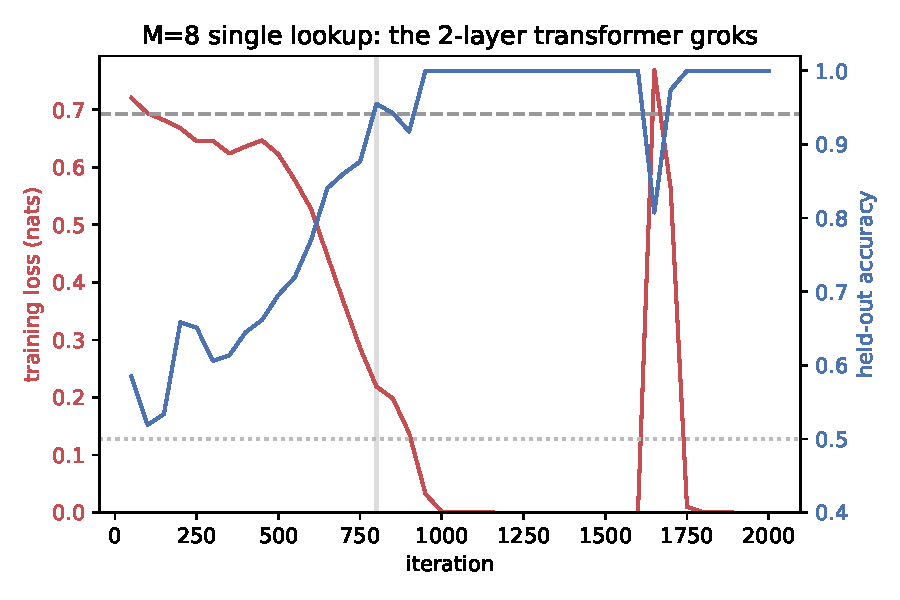
\includegraphics[width=0.85\linewidth]{figures/ch06-grokking.pdf}
  \caption{The two-layer transformer groks the $M=8$ single-lookup task.
  Training loss (left axis) holds at the random line $\ln 2 \approx 0.69$
  while the model searches, then collapses toward machine zero; held-out
  accuracy (right axis) tracks the same transition from chance to one. The
  brute-force MLP, by contrast, improves smoothly: fitting a lookup algorithm
  is a discrete jump, fitting an expert-per-address table is an
  interpolation.}
  \label{fig:ch06-grokking}
\end{figure}

The \textbf{MLP also reaches 100 percent}, and why is more interesting than
``it memorized.'' The MLP has 128 hidden units, and at $M=8$ with eight
possible addresses that is about sixteen hidden units per address. With that
budget it can learn a brute-force expert-per-address decomposition: a handful
of units that fire when the address equals $k$ and memory bit $k$ is one, with
the output layer summing the experts. That is an algorithm, not memorization,
but it scales linearly in the number of distinct addresses, so it starts to
break down once $2^A$ outgrows the hidden budget. The transformer is supposed
to scale linearly in $M$ regardless of $A$, because its attention is
content-addressable rather than expert-decomposed. \Cref{sec:scaling-puzzle}
takes the obvious next step and tests whether that scaling story holds.

\section{Multi-head attention and parallelism}\label{sec:multihead}

The single-head experiments already work, so what does adding heads buy?
Multi-head attention runs several attention operations in parallel within one
layer and combines them. Each head gets its own query, key, and value
projections acting on a slice of the model dimension, so the heads can
specialize: one might track a syntactic relation, another a long-range
dependency, another a specific token. An output projection $W_O$ recombines
the per-head read-outs. The real NumPy forward pass, from
\texttt{examples/transformer.py}, projects the input, splits it into heads,
runs the masked scaled-dot-product attention of \Cref{sec:attention-lookup}
per head, then merges and projects back:

\begin{lstlisting}
def forward(self, x):
    T, D = x.shape
    H, Dh = self.n_heads, self.head_dim
    scale = 1.0 / math.sqrt(Dh)

    q = self.W_q.forward(x)
    k = self.W_k.forward(x)
    v = self.W_v.forward(x)
    # Split into heads: (T, D) -> (H, T, Dh)
    Q = q.reshape(T, H, Dh).transpose(1, 0, 2)
    K = k.reshape(T, H, Dh).transpose(1, 0, 2)
    V = v.reshape(T, H, Dh).transpose(1, 0, 2)

    scores = (Q @ K.transpose(0, 2, 1)) * scale         # (H, T, T)
    mask = np.tril(np.ones((T, T)))
    scores = np.where(mask[None] > 0, scores, -1e9)
    attn = softmax(scores, axis=-1)                     # (H, T, T)
    heads_out = attn @ V                                # (H, T, Dh)
    merged = heads_out.transpose(1, 0, 2).reshape(T, D) # (T, D)
    return self.W_o.forward(merged)
\end{lstlisting}

The split is a reshape: the $d_{\text{model}}$ channels are partitioned into
$H$ contiguous blocks of $d_k = d_{\text{model}} / H$, each block its own
head, and the heads run independently before the merge concatenates them back.
For the pointer task at $M=8$, though, the lookup is conceptually a single
operation: one address to decode, one memory cell to read. A second head adds
no qualitatively new capability at this scale, and indeed a two-layer
two-head model converges to the same 100 percent accuracy as the two-layer
one-head model. The heads do not specialize because there is nothing here to
specialize on. That changes at larger $M$, where multiple heads turn out to
help for a reason the investigation in \Cref{sec:four-hypotheses} uncovers,
and it changes again on real language, where head specialization (induction
heads, copy heads, syntactic heads) is well documented. The synthetic task at
$M=8$ is simply not large enough to force it.

\section{Experiment 2: depth on a multi-hop lookup}\label{sec:exp-multihop}

To probe the depth story directly, switch to a pointer-to-pointer task. The
memory bit at the addressed position is combined with the address bits to form
a \emph{new} address, used for a second lookup, so the target is
\[
  y = m_{f(m_a,\, a)} ,
\]
where $f$ folds $m_a$ together with the lower bits of $a$ into the next
address. The exact combination is \texttt{make\_variant3} in
\texttt{examples/simple\_pointer\_dgp.py}; the point is that the target now
depends on two lookups composed in sequence. The model must decode the
address, read $m_a$, build the new address from that bit, and read memory
there. A two-layer transformer can in principle resolve the first lookup in
layer one and the second in layer two; a three-layer model has a layer to
spare. We train both on 20{,}000 examples for 2500 iterations:

\begin{center}
\begin{tabular}{@{}lrrr@{}}
\toprule
Model & Layers & Parameters & Test accuracy \\
\midrule
Transformer & 2 & 17{,}282 & \textbf{0.977} \\
Transformer & 3 & 25{,}826 & \textbf{0.995} \\
\bottomrule
\end{tabular}
\end{center}

The two-layer model gets close to perfect at 97.7 percent, and the three-layer
model essentially solves it at 99.5 percent; both grok within 2500 iterations.
The marginal gain from the third layer is small here because the task needs
only two hops, and a third layer is one more than that minimum. A three-hop
task would widen the gap between two and three layers. Even on this small
demonstration the trend is the one the depth-equals-composed-lookups story
predicts: more layers buy more hops. The next section tries to scale the
single-lookup task in the other direction, by memory size, and the clean
story breaks.
